\documentclass[letterpaper,landscape,9pt,fleqn]{extarticle}
%\usepackage[utf8]{inputenc}
%\usepackage[T1]{fontenc}
\usepackage{graphicx}
\usepackage{xcolor}
\usepackage{tikz}
\usepackage{url}
\usepackage{qrcode}
%\usetikzlibrary{shapes.geometric}
%\usetikzlibrary{calc}
%\usepackage{fourier}
\usepackage{graphicx,nicefrac}
\usepackage{isomath,upgreek,xcolor,comment}
\usepackage{pdfpages}
%\usepackage{tkz-euclide}
%\usetkzobj{all}
\pagestyle{empty}
\usepackage[activate={true,nocompatibility},final,tracking=true,kerning=true,factor=1100,stretch=10,shrink=10]{microtype}
\usepackage[american]{babel}
\usepackage{centernot}
\usepackage{amstext} % for \text macro
\usepackage{array}   % for \newcolumntype macro
\newcolumntype{L}{>{$}l<{$}} % math-mode version of "l" column type

\newcommand{\dom}{\mathrm{dom}} 
\newcommand{\range}{\mathrm{range}} 
\newcommand{\codom}{\mathrm{codom}}
\newcommand{\zero}{\mathrm{zero}} 
\newcommand{\reals}{\mathbf{R}} 
\newcommand{\ball}{\mathrm{ball}}
\newcommand{\integers}{\mathbf{Z}} 
\newcommand{\ssep}{\mid}
\newcommand{\arcsec}{\mathrm{arcsec}}
\newcommand{\arccsc}{\mathrm{arccsc}}
\newcommand{\arccot}{\mathrm{arccot}}
\newcommand{\glb}{\mathrm{glb}}
\newcommand{\lub}{\mathrm{lub}}
\newcommand{\length}{\mathrm{length}}
\usepackage{mathtools}
\DeclarePairedDelimiter{\parens}{\lparen}{\rparen}
\usepackage{amsmath,amssymb,textcomp}
\everymath{\displaystyle}

%\usepackage{times}
%\renewcommand\familydefault{\sfdefault}
%\usepackage{tgheros}
%\usepackage[defaultmono,scale=0.85]{droidmono}
%\usepackage{fourier}
\usepackage{multicol}
\setlength{\columnseprule}{0pt}
\setlength{\columnsep}{20.0pt}

\usepackage[]{enumerate}
\usepackage{expdlist}

\newenvironment{alphalist}{
  \begin{enumerate}[(a)]
    \addtolength{\itemsep}{-1.0\itemsep}}
  {\end{enumerate}}

\usepackage{geometry}
\geometry{letterpaper,left=0.4in,right=0.4in,top=0.4in,bottom=0.4in}

%\linespread{1.3}


% custom title
\makeatletter
\renewcommand*{\maketitle}{%
\noindent
\begin{minipage}{0.4\textwidth}

\begin{tikzpicture}
\node[rectangle,rounded corners=6pt,inner sep=10pt,fill=blue!50!black,text width= 0.95\textwidth] {\color{white}\Huge \@title};
\end{tikzpicture}
\end{minipage}
\hfill
\begin{minipage}{0.55\textwidth}
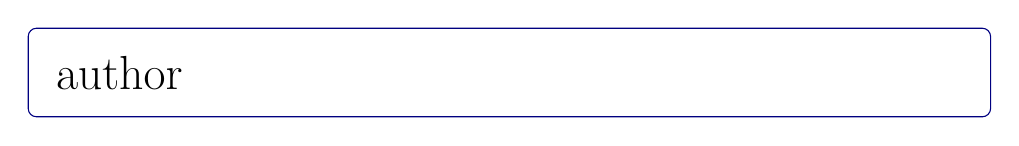
\begin{tikzpicture}
\node[rectangle,rounded corners=3pt,inner sep=10pt,draw=blue!50!black,text width= 0.95\textwidth] {\LARGE \@author};
\end{tikzpicture}
\end{minipage}
\bigskip\bigskip
}%
\makeatother

% custom section
\usepackage[explicit]{titlesec}
\newcommand*\sectionlabel{}
\titleformat{\section}
  {\gdef\sectionlabel{}
   \normalfont\sffamily\Large\bfseries\scshape}
  {\gdef\sectionlabel{\thesection\ }}{0pt}
  {
\noindent
\begin{tikzpicture}
\node[rectangle,rounded corners=3pt,inner sep=4pt,fill=blue!50!black,text width= 0.95\columnwidth] {\color{white}\sectionlabel#1};
\end{tikzpicture}
  }
\titlespacing*{\section}{0pt}{15pt}{10pt}


% custom footer
%\usepackage{fancyhdr}
%\makeatletter
%\pagestyle{fancy}
%\fancyhead{}
%\fancyfoot[C]{\footnotesize \textcopyright\ \@date\ \ \@author}
%\renewcommand{\headrulewidth}{0pt}
%\renewcommand{\footrulewidth}{0pt}
%\makeatother

\raggedbottom 
\raggedright
%\usepackage{tikz-3dplot}
\begin{document}

%\maketitle

\begin{multicols*}{3}

\section*{Greek characters}
\begin{tabular}{|L | L| L|} \hline
\mbox{Name} & \mbox{Symbol} & \mbox{Typical use(s)} \\ \hline
\mathrm{alpha} & \alpha  & \mbox{angle, constant} \\
\mathrm{beta} & \beta  & \mbox{angle, constant}  \\ 
\mathrm{gamma} & \gamma & \mbox{angle, constant} \\
\mathrm{delta} & \delta  & \mbox{limit definition}\\
\mathrm{epsilon} & \epsilon  \mbox{ or } \varepsilon & \mbox{limit definition} \\
\mathrm{theta}  & \theta  \mbox{ or } \vartheta &\mbox{angle}\\ 
\mathrm{pi} & \pi \mbox{ or } \uppi & \mbox{circular constant} \\
\mathrm{phi} & \phi \mbox{ or } \varphi  & \mbox{angle, constant} \\
\hline
\end{tabular}

\section*{Named sets}
\begin{minipage}[l]{0.15\textwidth}
    \begin{tabular}{|L | L |} \hline 
        \mathrm{empty\,\, set} & \varnothing \\ 
        \mathrm{real\,\, numbers} & \mathbf{R} \\
        \mathrm{ordered \, \, pairs }  & \mathbf{R}^2 \\
        \hline
    \end{tabular}
\end{minipage}
    \begin{minipage}[l]{0.15\textwidth}
        \begin{tabular}{|L | L |} \hline 
            \mathrm{integers } & \mathbf{Z} \\
            \mathrm{positive \,\,  integers } & \mathbf{Z}_{>0} \\ 
            \mathrm{positive \,\, reals} & \mathbf{R}_{>0} \\
            \hline
        \end{tabular}              
\end{minipage}

\section*{Set symbols}
\begin{minipage}[l]{0.15\textwidth}
    \begin{tabular}{|L | L|} \hline
        \mbox{Meaning}  & \mbox{Symbol} \\ \hline
        \mathrm{is \,\, a \,\, member} & \in \\
        \mathrm{subset}       & \subset \\
        \mathrm{intersection} & \cap \\ \hline
        \end{tabular}   
\end{minipage}
\begin{minipage}[l]{0.15\textwidth}
    \begin{tabular}{|L | L|} \hline
        \mbox{Meaning}  & \mbox{Symbol} \\ \hline
        \mathrm{union} & \cup  \\ 
        \mathrm{complement} & \mbox{superscript}^\mathrm{C} \\
        \mathrm{set \,\,  minus}  & \setminus \\ \hline
        \end{tabular}   
\end{minipage}
\section*{Intervals}
\begin{minipage}[c]{0.333\textwidth}
For numbers \(a\) and \(b\), we define the intervals:
\begin{align*}
 (a,b) &= \left\{x \in \reals \ssep a < x < b \right\}  \\
  [a,b) &= \{x  \in \reals  \ssep a \leq  x < b \} \\
   (a,b] &= \{x  \in \reals \ssep a <  x \leq  b \} \\
    [a,b]  &= \{x  \in \reals \ssep a \leq  x \leq  b \} \\
 %   (-\infty, a) &= \{x \mid x < a \} \\
 %   (-\infty, a] &= \{x \mid x \leq  a \} \\
 % (a, \infty)  &= \{x \mid a < x  \} \\
 %  [a, \infty)  &= \{x \mid a \leq  x  \} \\
\end{align*}  
\end{minipage}

\section*{Logic symbols}
\begin{minipage}[l]{0.15\textwidth}
    \begin{tabular}{|L | L|} \hline 
        \mbox{Meaning}  & \mbox{Symbol} \\ \hline 
        \mathrm{negation} &  \lnot   \\
        \mathrm{and} &  \land  \\
        \mathrm{or} &  \lor  \\
        \mathrm{implies} &  \implies \\ \hline    
    \end{tabular}   
\end{minipage}
\begin{minipage}[c]{0.15\textwidth}
    \begin{tabular}{|L | L|} \hline 
        \mbox{Meaning}  & \mbox{Symbol} \\ \hline 
        \mbox{equivalent} &  \equiv \\ 
        \mbox{iff} & \iff \\ 
        \mbox{for all} & \forall \\
        \mbox{there exists} & \exists \\ \hline
    \end{tabular}   
\end{minipage}

\begin{minipage}[t]{0.3333\textwidth}
\section*{Tautologies}
\vspace{-0.1in}
\begin{alignat*}{1}
    &\lnot \parens*{P \land Q} \equiv \lnot P \lor \lnot Q \\
    & \parens*{P \implies Q} \equiv \parens*{\lnot Q \implies \lnot P}\\
    &P \centernot \implies Q \equiv P \land \lnot Q \\
    &\parens*{P \iff Q} \equiv \parens*{\parens*{P \implies Q} \land \parens*{Q \implies P}} \\
    &\lnot \parens*{\forall \, x \in A}\parens*{P(x)} \equiv \parens*{\exists \, x \in A}\parens*{\lnot P \parens*{x}}  \\
    &\lnot \parens*{\exists \, x \in A} \parens*{P \parens*{x}} \equiv \parens*{\forall \, x \in A} \parens*{\lnot P \parens{x}}
 \end{alignat*}
\end{minipage}

\section*{Function notation}
\begin{tabular}{|L | L|} \hline 
    \dom(F) &   \mbox{domain of function } F \\
    \range(F) &   \mbox{range of function } F \\
    \mathrm{C}_{A} & \mbox{ set of continuous functions on set } A \\
    \mathrm{C}_{A}^1 & \mbox{ set of differentiable functions on set } A \\
    A \to B   & \mbox{set of functions from } A \mbox { to } B \\ \hline
\end{tabular}

 \section*{Generalized set operators}
 Each member of a set $\mathcal{C}$ is a set:
\begin{alignat*}{1}
    &\underset{A \in \mathcal{C}}{\bigcup} A = \left \{z \mid \parens*{\exists \, B  \in \mathcal{C} }\parens{z \in B} \right \}\\
    &\underset{A \in \mathcal{C}}{\bigcap} A = \left \{z \mid \parens*{\forall \, B \in \mathcal{C}}\parens{z \in B} \right \}
\end{alignat*}
Theorem: \(\underset{A \in \mathcal{C}}{\bigcup} A^\mathrm{C} = \parens*{\underset{A \in \mathcal{C}}{\bigcap} A}^\mathrm{C} \)
\section*{Functions applied to  sets}
Let $A \subset \dom(F)$ and $B \subset \range(F)$:
\begin{alignat*}{1}
    F(A) &= \{F(x) \mid x \in A \} \\
    F^{-1}(B) &= \{x \in \dom(F) \mid F(x) \in B \}
\end{alignat*}


\section*{Triangle inequalities}
For all $x,y \in \reals$, we have
\begin{alignat*}{1}
    |x+y| &\leq |x| + |y| \\
    \big | |x| - |y|  \big |  &\leq |x-y|    
\end{alignat*}
\section*{Floor and ceiling}
\vspace{-0.1in}
\noindent Definitions:
\begin{align*}
    \lfloor x \rfloor = \max \{k \in \integers \mid  k \leq x \} \\
    \lceil x \rceil = \min  \{k \in \integers \mid  k \geq x \}   
\end{align*}

\noindent Properties:
\begin{align*}
  % &\parens*{\forall x \in \reals} \parens*{\lfloor x \rfloor \leq x} \\
  % &\parens*{\forall x \in \reals} \parens*{\lceil x \rceil \geq x} \\
   & \parens*{\forall x \in \reals, n \in \integers} \parens*{x < n \iff  \lfloor x \rfloor < n}\\
   & \parens*{\forall x \in \reals, n \in \integers} \parens*{n < x \iff  n < \lceil  x \rceil}\\
\end{align*}
\vspace{-0.51in} 
\section*{Bounded sets}
\begin{description}[\itemsep=0em]
    \item[Bounded below] A set $A$ is \emph{bounded below} provided\\
        \((\exists \, M \in \reals)(\forall \, x \in A)(M \leq x)\).

    \item[Bounded above] The set $A$ is \emph{bounded above} provided\\
        \((\exists \, M \in \reals)(\forall \, x \in A)(x \leq M ) \).
        
    \item[Bounded] A set is \emph{bounded} if it is bounded below and bounded above.

\end{description}

\section*{Elementary function properties}
    \begin{description}[\itemsep=0em]
        \item[Increasing] \( \parens*{\forall \, x,y \in A} \parens*{x < y \implies F(x) \leq F(y)} \).
        For strictly increasing, replace $F(x) \leq F(y)$ with $F(x) < F(y)$.
        \item[Decreasing] \( \parens*{\forall \, x,y \in A} \parens*{x < y \implies F(x) \geq F(y)} \)
        For strictly decreasing, replace $F(x) \geq F(y)$ with $F(x) > F(y)$.
        \item[One-to-one] \( \parens*{\forall \, x,y \in \dom(F)} \parens*{F(x) = F(y) \implies x = y} \)
        \item[Subadditive] \( \parens*{\forall \, x,y \in \dom(F)} \parens*{F(x+y) \leq F(x) + F(y)} \)
        \item[Bounded above] \( \parens*{\exists \, M \in \reals} \parens*{\forall x \in \dom(F)} \parens*{F(x) \leq M} \)
        \item[Bounded below] \(\parens*{\exists \, M \in \reals} \parens*{\forall x \in \dom(F)} \parens*{M \leq F(x)}\)
    \end{description}

\section*{Topology}

\begin{description}[\itemsep=0em]
    \item[Open ball] $\ball(a, r) = \{x \in \reals \ssep -r + a< x < r+a \}$
  
    \item[Punctured ball] $\ball^\prime(a, r) = \ball(a, r) \setminus \{a\}$
  
    \item[Open set] A subset $A$ of $\reals$ is \emph{open} provided\\
        \(\left(\forall x \in A\right ) \left (\exists \, r \in \reals_{>0})(\ball(x,r) \subset A \right)\)
  
    \item[Closed set] A subset $A$ of $\reals$ is \emph{closed} provided \(\reals \setminus A\) is open.
  
    \item[Limit point] A number $a$ is a \emph{limit point} of a set $A$ provided
         \( \parens*{\forall \, r \in \reals_{>0}} \parens*{\ball^\prime(a, r) \cap A \neq \varnothing} \).
         
    \item[Boundary point] A number $a$ is a \emph{boundary point} of a set $A$ provided
    \( \parens*{\forall \, r \in \reals_{>0}} \parens*{\ball(a, r) \cap A \neq \varnothing \land 
    \ball(a, r) \cap A^{\mathrm{C}} \neq \varnothing } \).
   
    \item[Set closure] $\overline{A} = A \cup \mathrm{LP}(A)$, were $\mathrm{LP}(A)$ is the
    set of limit points of $A$.
    
    \item[Open cover] A set $\mathcal{C}$ is an open cover of a set $A$ provided 
     \begin{alphalist}
         \item every member of $\mathcal{C}$ is an open set
         \item $A \subset \underset{B \in \mathcal{C}}{\bigcup} B $
     \end{alphalist}

     \item[Compact] A set $A$ is compact provided for every 
     open cover $\mathcal{C}$ of $A$, there is a finite
     subset $\mathcal{C}^\prime$ of $\mathcal{C}$ such that
     $\mathcal{C}^\prime$ is an open cover of $A$.
     
    \end{description} 

\section*{Least and greatest bounds} 
For any subset $A$ of $\reals$:
\begin{description}[\itemsep=0em]
    \item[glb] $z = \glb(A)$ provided
    \begin{alphalist}
        \item $z$ is an lower bound for $A$
        \item if $x$ is a lower bound for $A$ then $x \leq z$
    \end{alphalist}
   \item[lub]  $z = \lub(A)$ provided
   \begin{alphalist}
       \item $z$ is an upper bound for $A$
       \item if $x$ is a upper bound for $A$ then $z \leq x$
   \end{alphalist}
\end{description}   
\section*{Sequences}
\begin{description}[\itemsep=0em]
\item[Bounded] A sequence $F$ is bounded if $\range(F)$ bounded.

\item[Monotone] A sequence is monotone if it either increases or
decreases.
\item[Cauchy] A sequence $F$ is Cauchy provided
\begin{alphalist}
    \item for every $\varepsilon \in \reals_{>0}$
    \item there is $n \in \integers$
    \item such that for all $k,\ell \in \integers_{>n}$
    \item $|F_k - F_\ell| < \varepsilon$
\end{alphalist}

\item[Converges] A sequence $F$ converges provided
\begin{alphalist}
    \item there is $L \in \reals$
    \item and $n \in \integers$
    \item such that for all $k \in \integers_{>n}$
    \item $|F_k - L | < \varepsilon$.
\end{alphalist}
\end{description}

\section*{Functions}   
\begin{description}[\itemsep=0em]
    \item[Continuous] A function $F$ is continuous at $a$ provided
    \begin{alphalist}
        \item $a \in \dom(F)$ and
        \item for every $\varepsilon \in \reals_{>0}$
        \item there is $\delta \in \reals_{>0}$
        \item such that for all $x \in \ball(a,\delta) \cap \dom(F)$
        \item we have $F(x) \in \ball(F(a), \epsilon)$.
    \end{alphalist}

    \item[Uniformly continuous]  A function $F$ is uniformly continuous on a set $A$ provided 
       \begin{alphalist}
          \item $A \subset \dom(F)$; and
          \item for every $\varepsilon \in \reals_{>0}$
          \item there is $\delta \in \reals_{>0}$
          \item such that for all $x,y  \in A$ and $ |x-y| < \delta$
          \item we have $|F(x) - F(y)| < \epsilon$.
       \end{alphalist} 
    \item[Limit]  A function $F$ has a limit toward $a$ provided
       \begin{alphalist}
          \item $a$ is a limit point of $\dom(F)$; and
          \item there is $L \in \reals$
          \item such that for every $\varepsilon \in \reals_{>0}$
          \item there is $\delta \in \reals_{>0}$
          \item such that for all $x \in \ball^\prime(a,\delta)$
          \item we have $F(x) \in \ball(L, \epsilon)$.
       \end{alphalist} 

    \item[Differentiable] A function $F$ is differentiable at $a$ provided
     \begin{alphalist}
    \item $a \in \dom(F)$; and
       \item there is $\phi \in \dom(F) \to \reals$
       \item such that $\phi$ is continuous at $a$ and
       \item $(\forall x \in \dom(F))(F(x) = F(a) + (x-a) \phi(x))$.
     \end{alphalist}
\end{description}

\section*{Riemann sums}
\begin{description}[\itemsep=0em]
    \item[Partition] A set $\mathcal{P}$ is a partition of an 
    interval $[a,b]$ provided
    \begin{alphalist}
        \item the set  $\mathcal{P}$ is finite
        \item every member of $\mathcal{P}$ is an open interval
        \item the members of $\mathcal{P}$ are pairwise disjoint
        \item $\underset{I \in \mathcal{P}} \bigcup \overline{I} = [a,b]$
    \end{alphalist}
\end{description}
Let $F$ be a bounded function on an interval $[a,b]$ and let
$\mathcal{P}$ be a partition of $[a,b]$. 
\begin{description}[\itemsep=0em]    
    \item[Lower sum] $\underline{S}(\mathcal{P}) = \sum_{I \in \mathcal{P}} \glb \parens*{F \parens*{\overline{I}}} \times  \length(I)$
    \item[Upper sum] $\overline{S}(\mathcal{P}) = \sum_{I \in \mathcal{P}} \lub \parens*{F \parens*{\overline{I}}} \times  \length(I)$
    \item[Riemann sum] $\sum_{I \in \mathcal{P}, x^\star \in \overline{I}} F \parens*{x^\star} \times  \length(I)$
\end{description}

\section*{Axioms}
\begin{description}
    \item[Completeness] Every nonempty subset $A$ of $\reals$ that is 
    bounded above has a least upper bound.
    \item[Well-ordering]  Every nonempty set of positive integers 
        contains a least element.
    \item[Induction] $\parens*{\forall n \in \integers_{\geq 0}}(P(n))$ if and only if
    $ P(0) \land \parens*{\forall n \in 
    \integers_{\geq 0}}  \parens*{P(n) \implies P(n+1)}$.
\end{description}

\section*{Named theorems}
    \begin{description}[\itemsep=0em]
    \item[Archimedean] \(\parens*{\forall x \in \reals} 
       \parens*{\exists n \in \integers}(n > x) \equiv \mbox{true}\).
    \item[Bolzano–Weirstrass] Every bounded real valued sequence has a convergent subsequence.
    \item[Heine–Borel] A subset of $\reals$ is compact iff it is closed and bounded.
    \item[Cauchy completeness]  Every Cauchy sequence in \(\reals\) converges. 
    \item[Monotone convergence] Every bounded monotone sequence converges.  
    \item[ Intermediate value theorem ] If $F \in \mathrm{C}_{[a,b]}$, then
    for all $y \in [\min(F(a),F(b)), \max(F(a),F(b))]$ there is
    $x \in [a,b]$ such that $F(x)=y$.      
    \item[Mean Value]  If $F \in \mathrm{C}_{[a,b]} \cap \mathrm{C}_{(a,b)}^1$, 
    there is $\xi \in (a,b) $ such that $(b-a) F^\prime(\xi) = F(b) - F(a)$.
\end{description}
\vfill
\noindent {Revised \today. Barton Willis is the author of this work. This work is
licensed under Attribution 4.0 International (CC BY 4.0) \,  \qrcode[height=0.15in]{https://creativecommons.org/licenses/by/4.0/}. For the current version of
this document, visit \, \qrcode[height=0.15in]{https://github.com/barton-willis/Math-100-200-level}}
\end{multicols*}%{3}

\end{document}